\documentclass{beamer}


\usepackage[french,english]{babel}

\usepackage[T1]{fontenc}

\usepackage[utf8]{inputenc}
\usepackage[linesnumbered,ruled,vlined]{algorithm2e}

\usetheme{Warsaw}
\title{Présentation stage}

\author{Clément Legrand}

\begin{document}


\begin{frame}[plain]
\titlepage
\end{frame}

\section{Présentation du problème}

\subsection{Vehicle Routing Problem}

\begin{frame}{Vehicle Routing Problem}
\begin{block}{Objectif}
Construire un ensemble de tournées qui respectent les règles suivantes:
\begin{itemize}
\item Chaque client doit être desservi par une et une seule tournée;
\item Chaque tournée doit partir et s'arrêter au dépôt;
\item La longueur du réseau est minimale.
\end{itemize}
\end{block}

\begin{block}{Données}
Les instances utilisées sont celles de la littérature. 

Pour chaque instance clients et dépôt sont définis.

\end{block}

\end{frame}

\begin{frame}{Exemple} 
Instance A-n32-k05 de la littérature.
\begin{center}
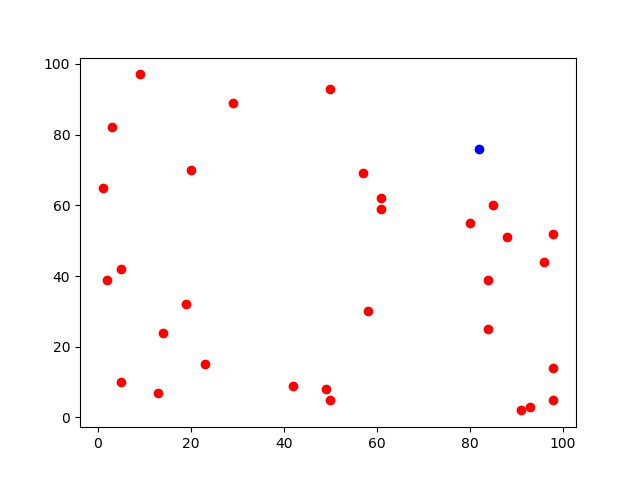
\includegraphics[scale=0.3]{Instance.png}
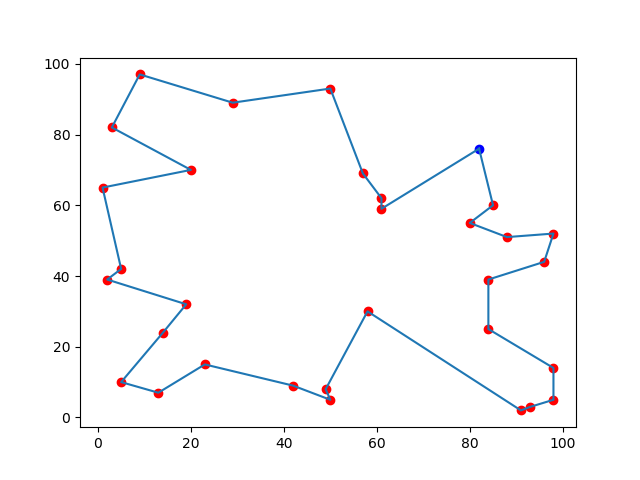
\includegraphics[scale=0.3]{solutionNoCapacity.png}
\end{center}
\end{frame}

\subsection{Capacitated VRP}

\begin{frame}{Ajout des demandes}
Problème plus intéressant : gestion des demandes des clients et de la capacité des véhicules.
\begin{block}{Nouvel objectif}
Une nouvelle règle vient s'ajouter aux règles précédentes:
\begin{itemize}
\item La demande totale sur une tournée ne doit pas excéder sa capacité.
\end{itemize}
\end{block}
\end{frame}

\begin{frame}{Exemple}
Reprenons A-n32-k05, en ajoutant les demandes des clients et une capacité limite:
\begin{center}
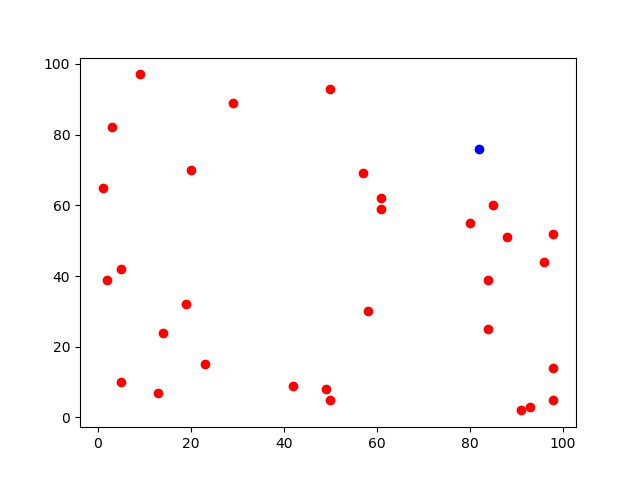
\includegraphics[scale=0.32]{Instance.png}
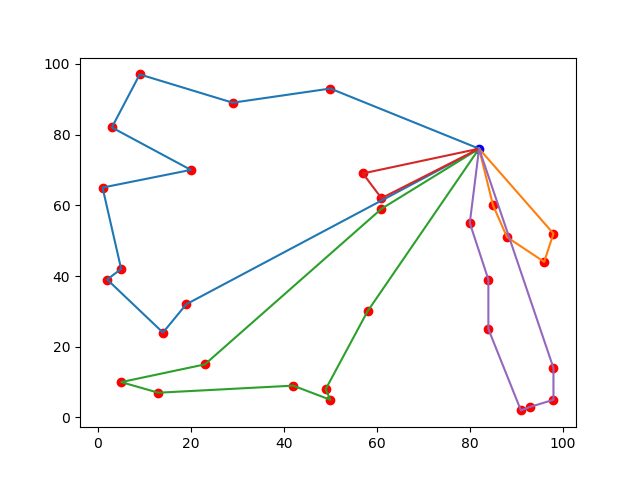
\includegraphics[scale=0.32]{solutionCapacity.png}
\end{center}
\end{frame}

\section{Contexte}

\subsection{Algorithme CW}

\begin{frame}{Algorithme Clarke \& Wright}
Algorithme glouton, qui permet de trouver une solution initiale pas trop mauvaise. 

\begin{block}{Description}
Pour chaque couple de clients $(i,j)$ on calcule le saving de $i$ et $j$ avec:
\begin{center}
$s(i,j) = c_{i0} + c_{0j} - \lambda c_{ij} + \mu \vert c_{i0} - c_{0j} \vert + \nu \frac{d_i + d_j}{\overline{d}}$
\end{center}
Tant que le saving maximal est positif:
\begin{itemize}
\item On prend $(i,j)$ tel que $s(i,j)$ soit maximal;
\item Les tournées qui contiennent $i$ et $j$ sont fusionnées (si possible);
\item On met $s(i,j) = 0$.
\end{itemize} 

\end{block}
\end{frame}

\subsection{Heuristique A \& S}

\begin{frame}{Heuristique A \& S}
Heuristique développée par Arnold et Sörensen en 2017. 

\underline{Intérêt}: heuristique simple à mettre en place, et performante.

\begin{algorithm}[H]
\DontPrintSemicolon % Some LaTeX compilers require you to use \dontprintsemicolon instead
\KwIn{L'instance considérée}
\KwOut{Une solution au problème I}
$Sol \gets Clarke and Wright$\;
\While {Pas 3 minutes depuis la dernière amélioration} {
	Calcul de la pire arête\;
	Application des opérateurs locaux\;
	\If {Nouvelle meilleure solution} {
		Mettre à jour $Sol$\;
	}
}
\Return{$Sol$}\;
\caption{{\sc AS} applique l'heuristique A\& S au problème considéré}
\label{algo:AS}
\end{algorithm}

\end{frame}

\begin{frame}{Pire arête}
\begin{exampleblock}{Pire arête}
La pire arète du graphe est l'arête $(i,j)$ qui maximise la fonction:
\begin{center}
$b(i,j) = \frac{[\lambda_w w(i,j) + \lambda_c c(i,j)] [\frac{d(i,j)}{max_{k,l}d(k,l)}] ^ {\frac{\lambda_d}{2}}}{1+p(i,j)}$
\end{center}
\end{exampleblock}

\begin{figure}
\centering
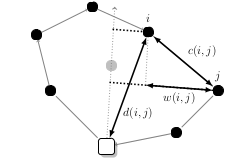
\includegraphics[scale=0.5]{metrics.png}
\end{figure}

\end{frame}

\begin{frame}{Opérateurs locaux}
\begin{block}{Ejection-chain}
Cet opérateur va essayer de déplacer au plus $l$ clients sur des tournées plus adaptées. 
\end{block}
\begin{block}{Cross-exchange}
Essaie d'échanger deux séquences de clients entre deux tournées. 
\end{block}
\begin{figure}
	\centering
	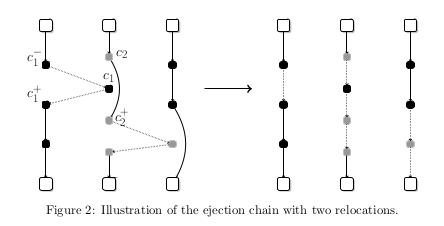
\includegraphics[scale=0.3]{ejection_chain.png}
	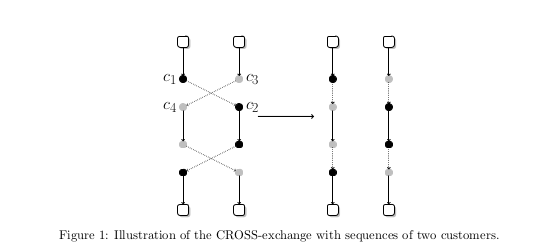
\includegraphics[scale=0.3]{cross_exchange.png}
\end{figure}

\end{frame}

\begin{frame}{Opérateurs locaux}
\begin{block}{Lin-Kernighan}
\begin{itemize}
\item Utilisé en général pour TSP;
\item Optimisation intra-tournée (chaque tournée est améliorée indépendamment des autres).
\end{itemize}
\end{block}
\begin{figure}
	\centering
	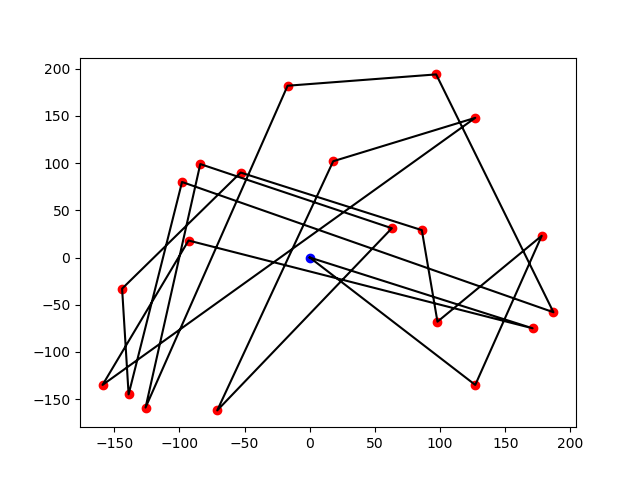
\includegraphics[scale=0.3]{test4_20_init.png}
	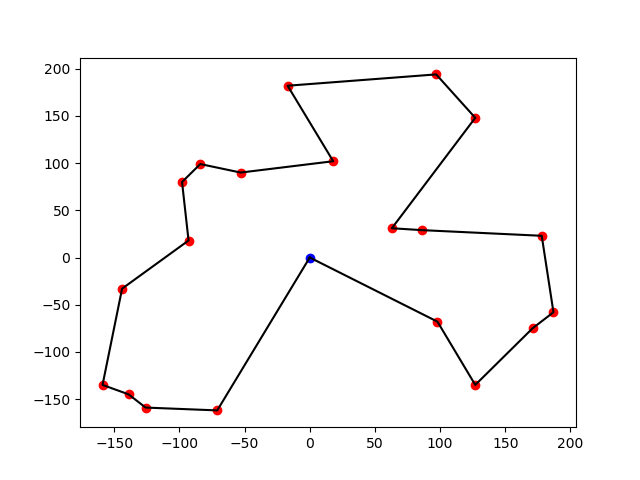
\includegraphics[scale=0.3]{test4_20_LKopt.png}
\end{figure} 
\end{frame}

\subsection{Motivation}

\begin{frame}{Intégration de connaissances}
\begin{block}{Objectif}
Améliorer les performances de l'heuristique en y intégrant de la connaissance.
\end{block}

\begin{exampleblock}{Idée}
Utiliser les résultats de CW pour tenter de prédire des arêtes qui appartiendront à la meilleure solution.
\end{exampleblock}
\end{frame}

\section{Résultats}

\subsection{Algorithme de base}

\begin{frame}{Description}
L'algorithme utilisé s'inspire de l'heuristique A\&S. 
\begin{block}{Modifications}
\begin{itemize}
\item On applique LK à la solution initiale;
\item Les opérateurs explorent les voisinages de manière aléatoire;
\item On repart de la dernière meilleure solution obtenue, après N/2 itérations sans améliorations.
\end{itemize}
\end{block}
\end{frame}

\begin{frame}{Résultats}

\end{frame}

\subsection{Extraction de connaissances}

\begin{frame}{Description}
Création d'une base de solutions pour extraire des connaissances.
\begin{block}{Protocole}
\begin{itemize}
\item Génération d'une base de 100 solutions aléatoirement;
\item On garde les solutions qui ont un coût inférieur à $c_{min} + (c_{max}-c_{min})\frac{10}{100}$ : qualité privilégiée. On appelle cette base Qual$_{10}$;
\item Pour chaque arête (i,j) (resp (j,i) si j<i), on incrémente la valeur de MAT[i][j] (resp MAT[j][i]);
\item On ne conserve que les $n/2$ premières arêtes dans la matrice.
\end{itemize}
\end{block}
\end{frame}

\begin{frame}{Résultats}

\end{frame}

\subsection{Intégration des connaissances}

\begin{frame}{Description}

\end{frame}

\begin{frame}{Résultats}

\end{frame}

\end{document}